% Source: tex/chapters/ch05/06_テスト技法.tex
\subsubsection{仕様ベース技法}
仕様ベース技法は、SUT の入力と出力、要求、仕様、モデルに基づいてテストケースを選ぶ。内部コードを知らなくても使えるため、ブラックボックス技法とも呼ばれる。

\paragraph{同値分割}
同値分割は、入力領域を同じように扱えると考えられる部分集合に分け、各集合から代表値を選ぶ技法である。たとえば、年齢が 0 から 120 まで有効なら、有効範囲、下限未満、上限超過などに分ける。目的は、無数の入力を少数の代表例に縮約することである。

\paragraph{境界値分析}
境界値分析は、入力範囲の境界付近に欠陥が集中しやすいという経験に基づき、下限、上限、その直前直後を選ぶ技法である。範囲外の値を使って堅牢性を見る場合もある。

\begin{figure}[htbp]
\centering
\IfFileExists{assets/generated_figures/ch05/fig-ch05-07.png}{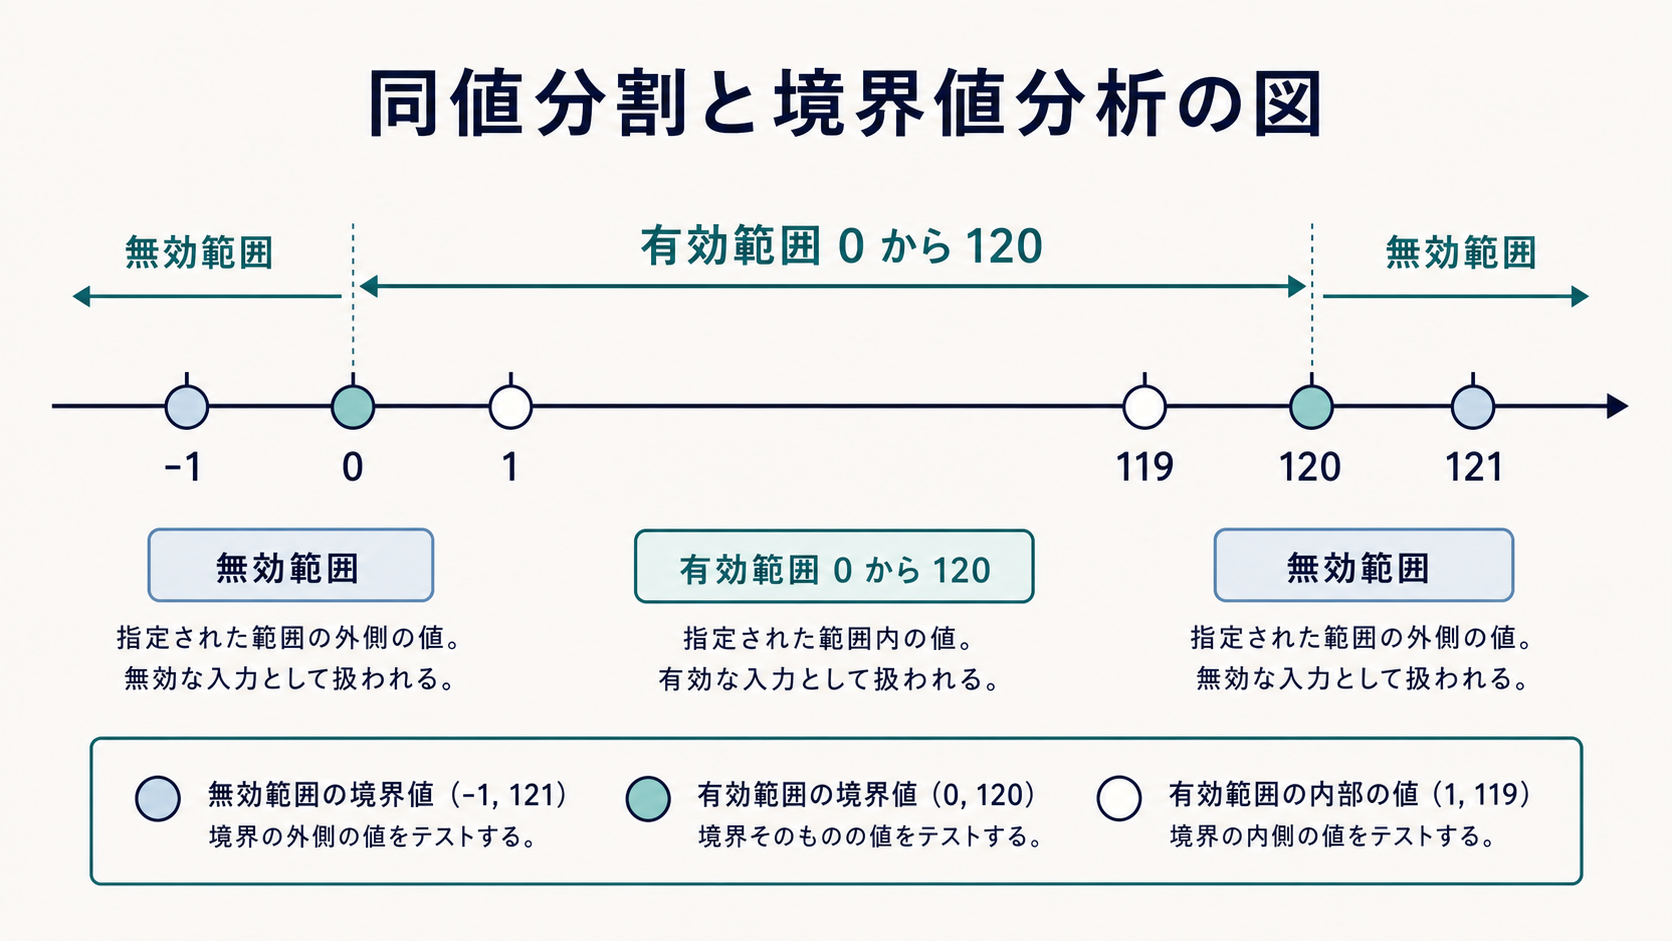
\includegraphics[width=0.96\linewidth]{assets/generated_figures/ch05/fig-ch05-07.png}}{\fbox{\parbox[c][48mm][c]{0.9\linewidth}{\centering 画像生成待ち\\同値分割と境界値分析の図}}}
\caption{同値分割と境界値分析の図}
\label{fig:ch05-07}
\end{figure}

\paragraph{構文テスト}
構文テストは、形式言語で書かれた仕様や入力文法に基づいてテストケースを導く技法である。仕様が形式的であれば、機能テストケースの自動生成や期待結果の判定に使いやすい。

\paragraph{組合せテスト技法}
組合せテストは、入力値や条件の組合せを体系的に選ぶ技法である。すべての組合せを試すと数が爆発するため、ペアワイズテストのように、任意の二つのパラメータの組合せはすべて含めるという基準を使うことが多い。

\paragraph{決定表}
決定表は、条件と動作の組合せを表にして、論理関係を明示する技法である。複数条件によって結果が変わる業務規則に向いている。各条件組合せからテストケースを導けるため、抜け漏れの発見にも役立つ。

\paragraph{原因結果グラフ}
原因結果グラフは、入力条件である原因と、出力や動作である結果の関係を論理グラフとして表す技法である。仕様分析、入力条件の整理、結果条件の特定に役立つ。

\paragraph{状態遷移テスト}
状態遷移テストは、SUT を有限状態機械として表し、状態と遷移をカバーするようにテストケースを作る技法である。画面遷移、通信プロトコル、注文状態、予約状態など、状態によって振る舞いが変わる対象に向いている。

\begin{figure}[htbp]
\centering
\IfFileExists{assets/generated_figures/ch05/fig-ch05-08.png}{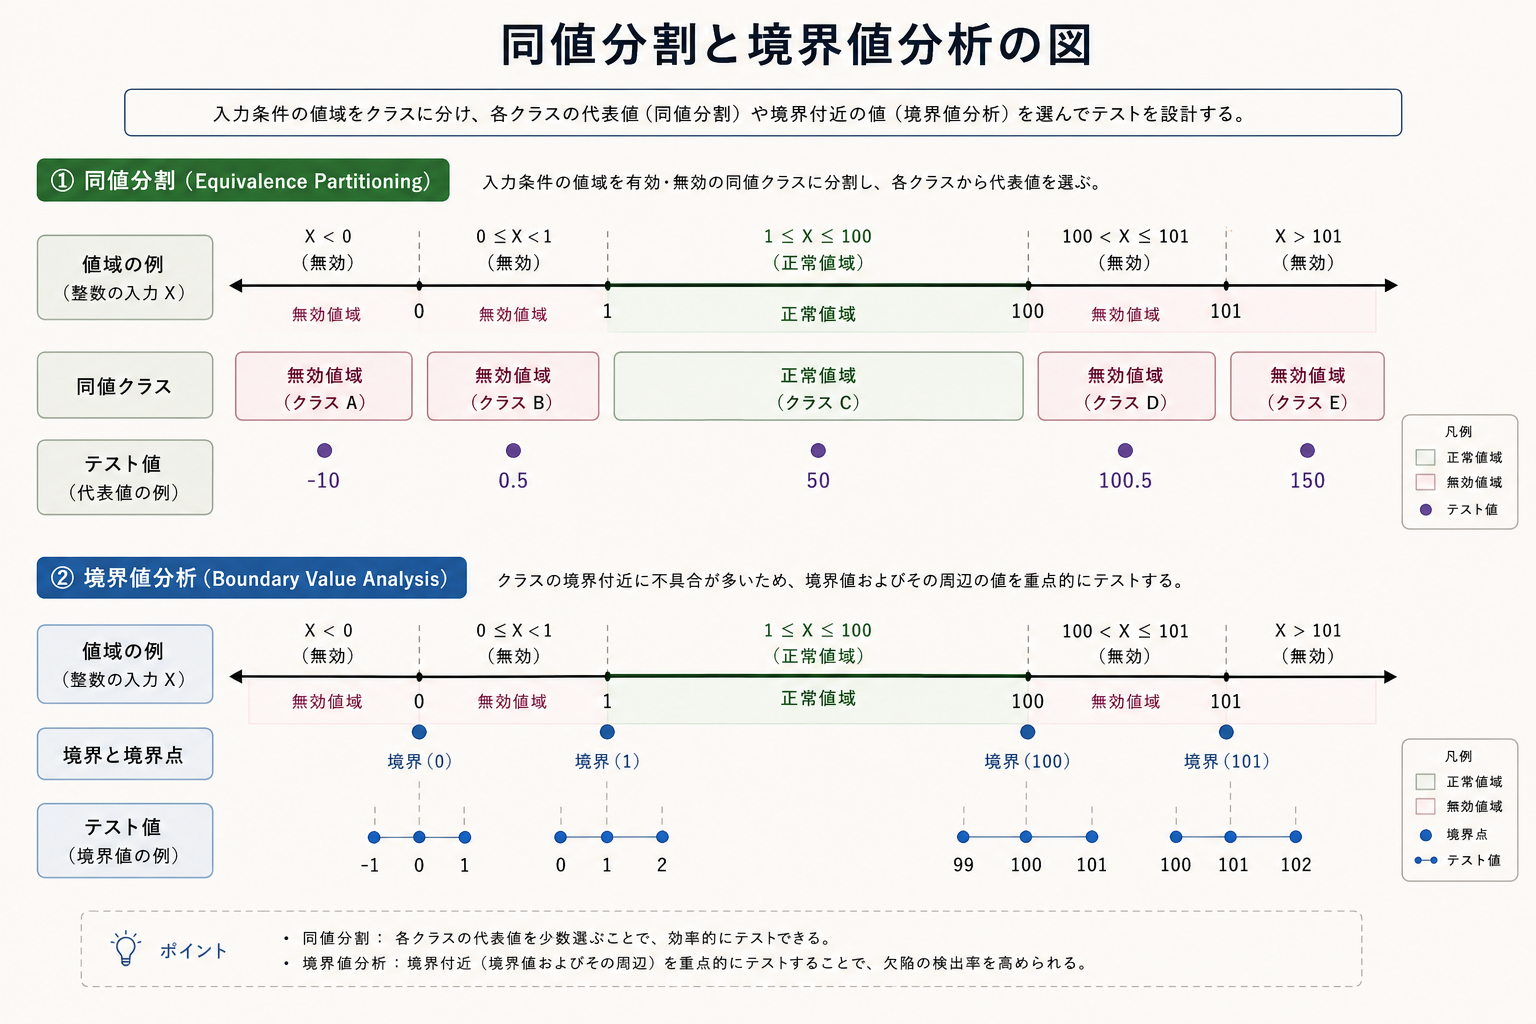
\includegraphics[width=0.96\linewidth]{assets/generated_figures/ch05/fig-ch05-08.png}}{\fbox{\parbox[c][48mm][c]{0.9\linewidth}{\centering 画像生成待ち\\状態遷移テストの図}}}
\caption{状態遷移テストの図}
\label{fig:ch05-08}
\end{figure}

\paragraph{シナリオベーステスト}
シナリオベーステストは、利用者やシステムがたどる一連の行動をモデル化し、その流れに沿ってテストケースを作る技法である。通常の流れだけでなく、代替流、例外流も扱う。業務プロセステストやワークフローモデルを使うテストもこの考え方に含まれる。

\paragraph{ランダムテスト}
ランダムテストは、入力領域からランダムにテストケースを選ぶ技法である。単純な自動化に向いているが、入力領域がわかっている必要がある。不正入力や予期しないデータを大量に与えるファズテストは、セキュリティ分野でよく用いられる。

\paragraph{証拠に基づく技法}
証拠に基づく技法は、厳密な調査手順で得た知見をテストに反映する考え方である。問いを立て、利用できる証拠を集め、批判的に分析する。体系的マッピング研究や体系的レビューは、既存研究や実務知見を整理する手段である。

\paragraph{例外強制テスト}
例外強制テストは、データ例外、操作例外、オーバーフロー、保護例外、アンダーフローなど、あらかじめ決めた例外やエラーを SUT が扱えるかを確認する。多くの場合、負のシナリオを使い、エラーメッセージや回復動作を確認する。
